\subsection{x86}

\subsubsection{\NonOptimizing MSVC}

Result (MSVC 2010):

\lstinputlisting[caption=MSVC 2010]{patterns/08_switch/1_few/few_msvc.asm}

Our function with a few cases in switch() is in fact analogous to this construction:

\lstinputlisting[label=switch_few_ifelse]{patterns/08_switch/1_few/few_analogue.c}

\myindex{\CLanguageElements!switch}
\myindex{\CLanguageElements!if}

If we work with switch() with a few cases it is impossible to be sure if it was
a real switch() in the source code, or just a pack of if() statements.
\myindex{\SyntacticSugar}

This implies that switch() is like syntactic sugar for a large number of nested if()s.

There is nothing especially new to us in the generated code,
with the exception of the compiler moving input variable $a$ to a temporary local variable \TT{tv64}
\footnote{Local variables in stack are prefixed with \TT{tv}---that's how MSVC names internal variables for its needs}.

If we compile this in GCC 4.4.1, we'll get almost the same result, even with maximal optimization
turned on (\Othree option).

\subsubsection{\Optimizing MSVC}

% TODO separate various kinds of \TT
% idea: enclose command lines in a specific environment, like \cmdline{} 
% assembly instructions in \asm{} (now both \TT and \q{} are used),
% variables in,  like \var{}
% messages (string constants) in something else, like \strconst
% to separate them all. Now they all use \TT, which is not best
% \INS{} for all instructions including operands? --DY
Now let's turn on optimization in MSVC (\Ox): \TT{cl 1.c /Fa1.asm /Ox}

\label{JMP_instead_of_RET}
\lstinputlisting[caption=MSVC]{patterns/08_switch/1_few/few_msvc_Ox.asm}

Here we can see some dirty hacks.

\myindex{x86!\Instructions!JZ}
\myindex{x86!\Instructions!JE}
\myindex{x86!\Instructions!SUB}

First: the value of $a$ is placed in \EAX and 0 is subtracted from it. Sounds absurd, but it is done to check if 
the value in \EAX was 0. If yes, the \ZF flag is to be set (e.g. subtracting from 0 is 0) 
and the first conditional jump \JE (\IT{Jump if Equal} or synonym \JZ~---\IT{Jump if Zero}) is to be triggered 
and control flow is to be passed to the \TT{\$LN4@f} label, where the \TT{'zero'} message is being printed. 
If the first jump doesn't get triggered, 1 is subtracted from the input value and if at some stage the result is 0, 
the corresponding jump is to be triggered.

And if no jump gets triggered at all, the control flow passes to \printf with string argument \TT{'something unknown'}.

\label{jump_to_last_printf}
\myindex{\Stack}

Second: we see something unusual for us: a string pointer is placed into the $a$ variable, and 
then \printf is called not via \CALL, but via \JMP. There is a simple explanation for that: 
the \gls{caller} pushes a value to the stack and calls our function via \CALL. 
\CALL itself pushes the return address (\ac{RA}) to the stack and does an unconditional jump to our function address. 
Our function at any point of execution (since it do not contain any instruction that moves the stack 
pointer) has the following stack layout:

\begin{itemize}
\item\ESP\EMDASHpoints to \ac{RA}
\item\TT{ESP+4}\EMDASHpoints to the $a$ variable 
\end{itemize}

On the other side, when we need to call \printf here we need exactly the same stack 
layout, except for the first \printf argument, which needs to point to the string. 
And that is what our code does.

It replaces the function's first argument with the address of the string and 
jumps to \printf, as if we didn't call our function \ttf, but directly \printf.
\printf prints a string to \gls{stdout} and then executes the \RET instruction, which POPs 
\ac{RA} from the stack and control flow is returned not to \ttf but rather to \ttf's \gls{callee}, 
bypassing the end of the \ttf function.

\myindex{\CStandardLibrary!longjmp()}
\newcommand{\URLSJ}{\href{http://go.yurichev.com/17121}{wikipedia}}

All this is possible because \printf is called right at the end of the \ttf function in all cases. 
In some way, it is similar to the \TT{longjmp()}\footnote{\URLSJ} function.
And of course, it is all done for the sake of speed.

A similar case with the ARM compiler is described in \q{\PrintfSeveralArgumentsSectionName}
section, here~(\myref{ARM_B_to_printf}).

\clearpage
\myparagraph{\olly}

Since this example is tricky, let's trace it in \olly.

\olly can detect such switch() constructs, and it can add some useful comments.
\EAX is 2 in the beginning, that's the function's input value: 

\begin{figure}[H]
\centering
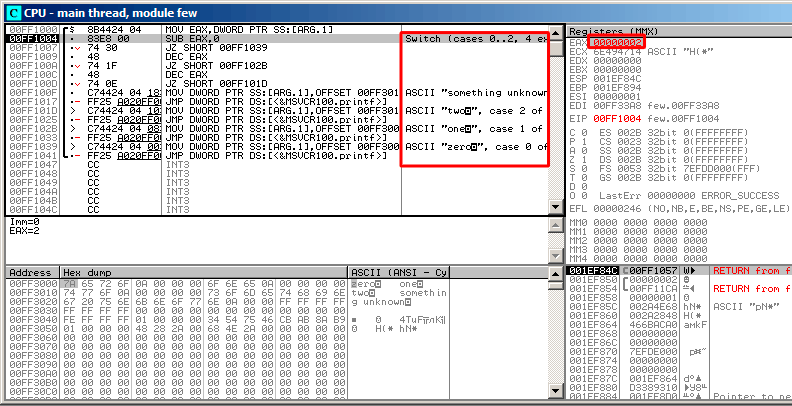
\includegraphics[scale=\FigScale]{patterns/08_switch/1_few/olly1.png}
\caption{\olly: \EAX 
now contain the first (and only) function argument}
\label{fig:switch_few_olly1}
\end{figure}

\clearpage
0 is subtracted from 2 in \EAX. 
Of course, \EAX still contains 2.
But the \ZF flag is now 0, indicating that the resulting value is non-zero:

\begin{figure}[H]
\centering
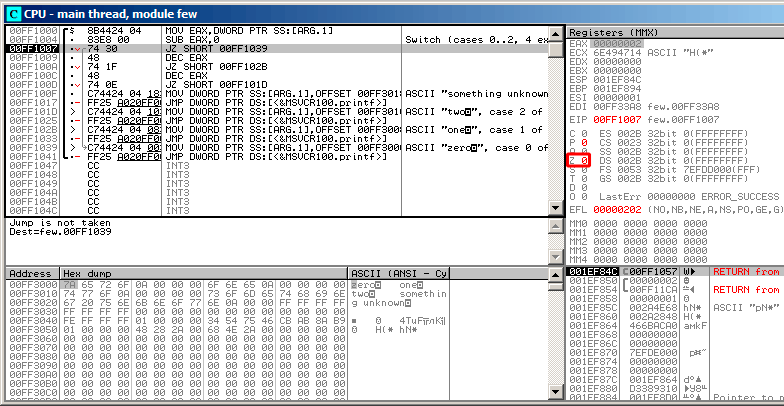
\includegraphics[scale=\FigScale]{patterns/08_switch/1_few/olly2.png}
\caption{\olly: \SUB executed}
\label{fig:switch_few_olly2}
\end{figure}

\clearpage
\DEC is executed and \EAX now contains 1. 
But 1 is non-zero, so the \ZF flag is still 0:

\begin{figure}[H]
\centering
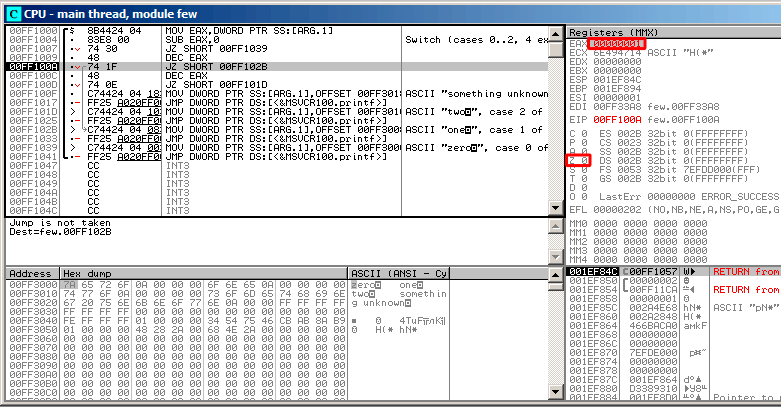
\includegraphics[scale=\FigScale]{patterns/08_switch/1_few/olly3.png}
\caption{\olly: first \DEC executed}
\label{fig:switch_few_olly3}
\end{figure}

\clearpage
Next \DEC is executed. 
\EAX is finally 0 and the \ZF flag gets set, because the result is zero:

\begin{figure}[H]
\centering
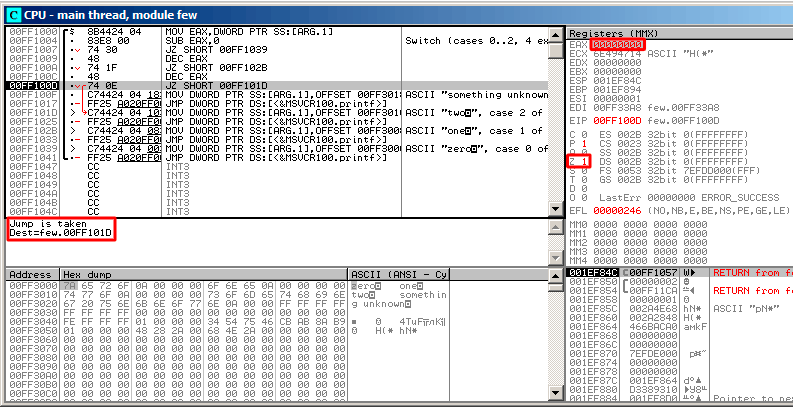
\includegraphics[scale=\FigScale]{patterns/08_switch/1_few/olly4.png}
\caption{\olly: second \DEC executed}
\label{fig:switch_few_olly4}
\end{figure}

\olly shows that this jump is to be taken now.

\clearpage
A pointer to the string \q{two} is to be written into the stack now:

\begin{figure}[H]
\centering
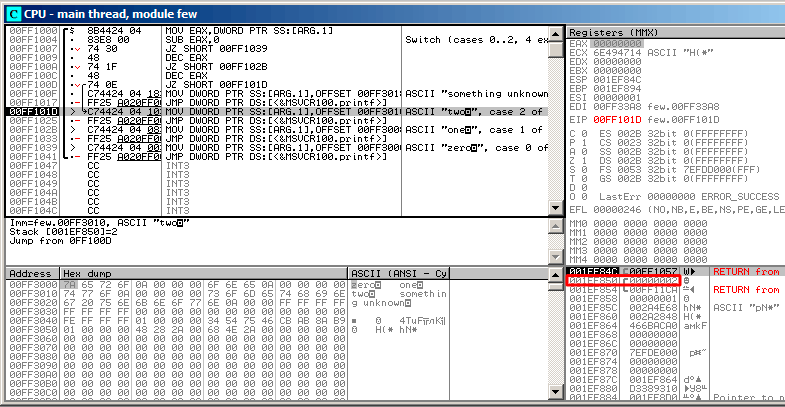
\includegraphics[scale=\FigScale]{patterns/08_switch/1_few/olly5.png}
\caption{\olly: 
pointer to the string is to be written at the place of the first argument}
\label{fig:switch_few_olly5}
\end{figure}

% TODO: homogenize numbers
% now they are inconsistent: sometimes plain text, sometimes in math mode
% some kind of \expr{} both for numbers and expressions? --DY
Please note: the current argument of the function is 2 and 2 is now in the stack at the address \TT{0x001EF850}.

\clearpage
\MOV writes the pointer to the string at address \TT{0x001EF850} (see the stack window).
Then, jump happens.
This is the first instruction of the \printf function in MSVCR100.DLL (This example was compiled with /MD switch): 

\begin{figure}[H]
\centering
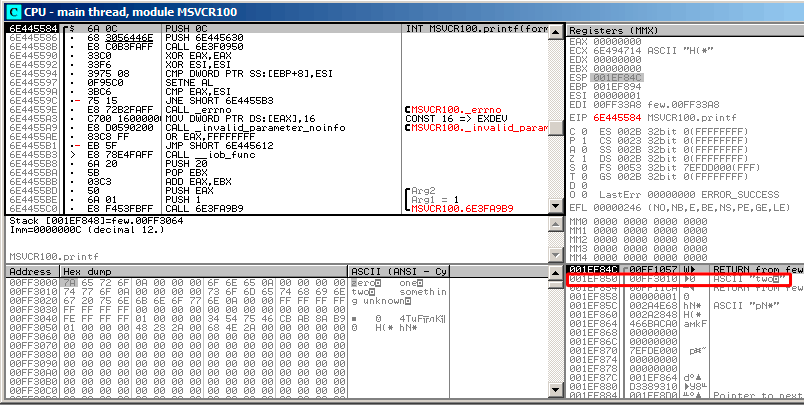
\includegraphics[scale=\FigScale]{patterns/08_switch/1_few/olly6.png}
\caption{\olly: first instruction of \printf \InENRU MSVCR100.DLL}
\label{fig:switch_few_olly6}
\end{figure}

Now \printf treats the string at \TT{0x00FF3010} as its only argument and prints the string.

\clearpage
This is the last instruction of \printf:

\begin{figure}[H]
\centering
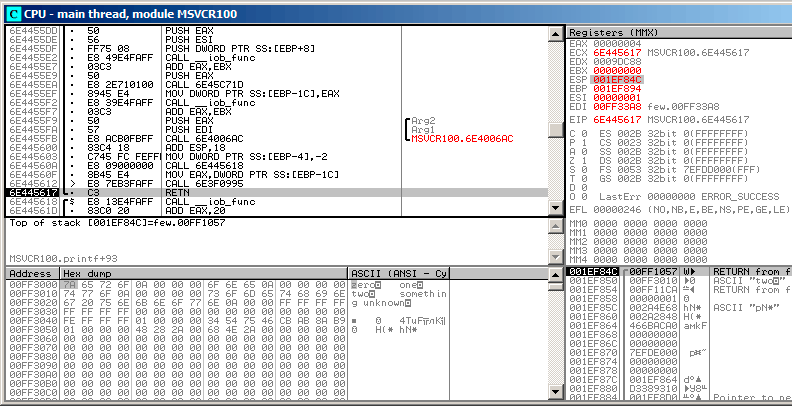
\includegraphics[scale=\FigScale]{patterns/08_switch/1_few/olly7.png}
\caption{\olly: last instruction of \printf in MSVCR100.DLL}
\label{fig:switch_few_olly7}
\end{figure}

The string \q{two} was just printed to the console window.

\clearpage
Now let's press F7 or F8 (\stepover) and return\dots not to \ttf , but rather to \main:

\begin{figure}[H]
\centering
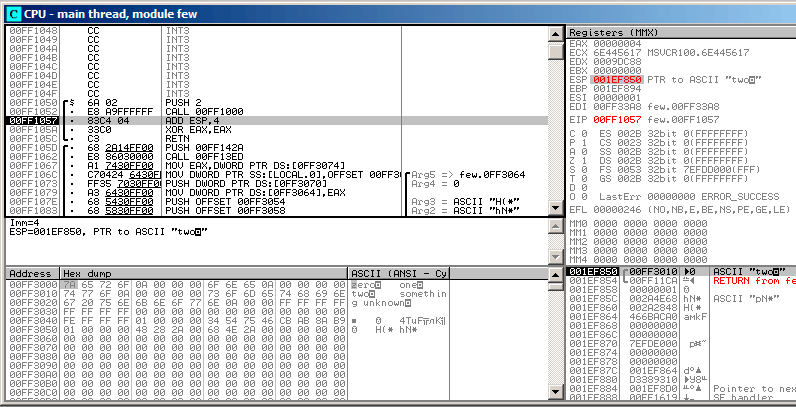
\includegraphics[scale=\FigScale]{patterns/08_switch/1_few/olly8.png}
\caption{\olly: return to \main}
\label{fig:switch_few_olly8}
\end{figure}

Yes, the jump was direct, from the guts of \printf to \main.
Because \ac{RA} in the stack points not to some place in \ttf , but rather to \main.
And \CALL \TT{0x00FF1000} was the actual instruction which called \ttf.



